\documentclass{article}
\usepackage{civ}
\newcommand*{\tabbox}[2][t]{%
    \vspace{0pt}\parbox[#1][3.7\baselineskip]{1cm}{\strut#2\strut}}
\title{CIV102: Problem Set \#5}
\author{QiLin Xue \\ \href{mailto:qilin.xue@mail.utoronto.ca}{qilin.xue@mail.utoronto.ca} \\ TA: Michel}
\everymath{\displaystyle}

\date{\today}
\usepackage{mathrsfs}
\usetikzlibrary{arrows}
\usepackage{siunitx}
\usepackage{wasysym}
\usetikzlibrary{calc}
\usepackage{xcolor}
\setlength\parindent{0pt}
% \setlength\extrarowheight{10pt}
\renewcommand{\arraystretch}{2}
\usepackage{adjustbox}
\begin{document}
\maketitle
\section{Problem One: Joint Loads}
Denote the position of each joint (and including the rightmost pin) with respect to the previous as $\Delta x_i$. For example, the position of $B$ relative to the previous joint is $\Delta x_2=4.5\si{\meter}$. Thus for an arbitrary joint $i$ where $1 \le i \le 9$, the load that it carries is given by:
\begin{equation}
    W_i = (2 \si{\meter} \cdot 9.2\si{\kilo\pascal})\frac{\Delta x_i+\Delta x_{i+1}}{2}=9.8(\Delta x_i+\Delta x_{i+1})
    \label{eq:}
\end{equation}
where $x$ is in meters. Thus:
\begin{align}
    W_A=W_1 = 9.2( 5+4.5 ) &= \boxed{ 87.4 \si{\kilo\newton}} \\
    W_B=W_2 = 9.2( 4.5+ 4) &= \boxed{ 78.2 \si{\kilo\newton}} \\
    W_C=W_3 = 9.2( 4+ 3.5) &= \boxed{ 69.0 \si{\kilo\newton}} \\
    W_D=W_4 = 9.2( 3.5+ 5.5) &= \boxed{ 82.8\si{\kilo\newton}} \\
    W_E=W_5 = 9.2( 5.5+ 5.5) &= \boxed{ 101.2\si{\kilo\newton}} \\
    W_F=W_6 = 9.2( 5.5+ 3.5) &= \boxed{82.8\si{\kilo\newton}} \\
    W_G=W_7 = 9.2( 3.5+ 4) &= \boxed{69.0\si{\kilo\newton}} \\
    W_H=W_8 = 9.2( 4+ 4.5) &= \boxed{ 78.2\si{\kilo\newton}} \\
    W_I=W_9 = 9.2( 4.5+5 ) &= \boxed{ 87.4\si{\kilo\newton}}
\end{align}
Note that due to the symmetry, we only need to calculate the forces on half of the bridge.

\newpage
\section{Problem Two: A Tikz Nightmare}
Let's first draw a diagram. The roller at $M$ is denoted in blue.
\begin{center}
    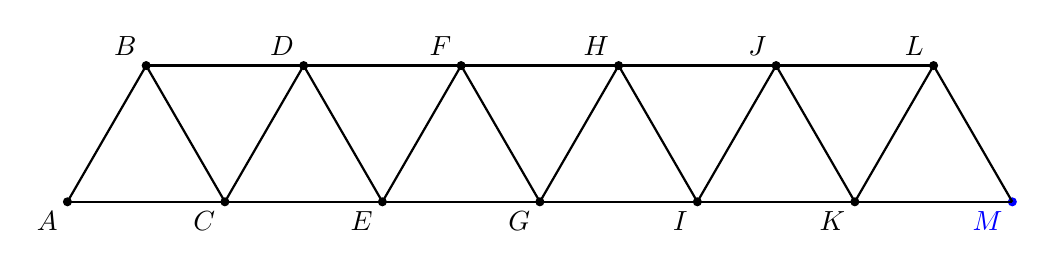
\begin{tikzpicture}
        \coordinate (A) at (0,0);
        \coordinate (C) at (2,0);
        \coordinate (E) at (4,0);
        \coordinate (G) at (6,0);
        \coordinate (I) at (8,0);
        \coordinate (K) at (10,0);
        \coordinate (M) at (12,0);

        \coordinate (B) at (1,1.73);
        \coordinate (D) at (3,1.73);
        \coordinate (F) at (5,1.73);
        \coordinate (H) at (7,1.73);
        \coordinate (J) at (9,1.73);
        \coordinate (L) at (11,1.73);

        \draw[fill=black] (A) circle (0.05) node[below left] {$A$};
        \draw[fill=black] (B) circle (0.05) node[above left] {$B$};
        \draw[fill=black] (C) circle (0.05) node[below left] {$C$};
        \draw[fill=black] (D) circle (0.05) node[above left] {$D$};
        \draw[fill=black] (E) circle (0.05) node[below left] {$E$};
        \draw[fill=black] (F) circle (0.05) node[above left] {$F$};
        \draw[fill=black] (G) circle (0.05) node[below left] {$G$};
        \draw[fill=black] (H) circle (0.05) node[above left] {$H$};
        \draw[fill=black] (I) circle (0.05) node[below left] {$I$};
        \draw[fill=black] (J) circle (0.05) node[above left] {$J$};
        \draw[fill=black] (K) circle (0.05) node[below left] {$K$};
        \draw[fill=black] (L) circle (0.05) node[above left] {$L$};
        \draw[color=blue,fill=blue] (M) circle (0.05) node[below left] {$M$};

        \draw[thick] (A) -- (C) -- (E) -- (G) -- (I) -- (K) -- (M);
        \draw[thick] (B) -- (D) -- (F) -- (J) -- (L);
        \draw[thick] (A) -- (B) -- (C) -- (D) -- (E) -- (F) -- (G) -- (H) -- (I) -- (J) -- (K) -- (L) -- (M);
    \end{tikzpicture}
\end{center}
We can abuse the symmetry of the bridge to develop a recursive solution. The weight each joint is responsible for is $W=70\si{\kilo\newton\per\meter} \cdot 5\si{\meter} = 350\si{\kilo\newton}$ and the edge joints are each responsible for half, or $175\si{\kilo\newton}$. But there is also an upwards reaction force equal to $\frac{1}{2} 70\si{\kilo\newton\per\meter} \cdot 30\si{\meter} = 1050\si{\kilo\newton}$ for a total reaction force of $875\si{\kilo\newton}$ upwards. Then we can draw a free body diagram for an arbitrary joint $i$:
\begin{center}
    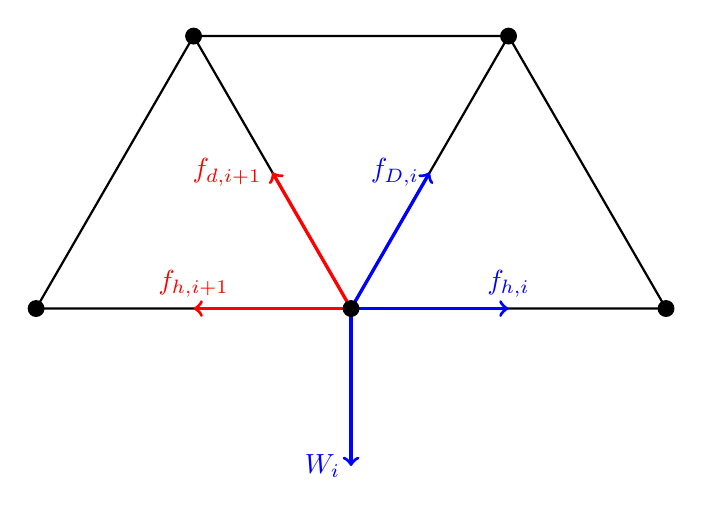
\begin{tikzpicture}[scale=2]
        \coordinate (A) at (0,0);
        \coordinate (B) at (1,1.73);
        \coordinate (C) at (2,0);
        \coordinate (D) at (3,1.73);
        \coordinate (E) at (4,0);


    
        \draw[thick] (A) -- (B) -- (D) -- (E) -- (C) -- (A);
        \draw[thick] (B) -- (C) -- (D);

        \draw[very thick, blue, ->] (C) -- ++(0,-1) node[left] {$W_i$};
        \draw[very thick, blue, ->] (C) -- ($(C) !0.5! (D)$) node[left] {$f_{D,i}$};
        \draw[very thick, blue, ->] (C) -- ($(C) !0.5! (E)$) node[above] {$f_{h,i}$};
        \draw[very thick, red, ->] (C) -- ($(C) !0.5! (B)$) node[left] {$f_{d,i+1}$};
        \draw[very thick, red, ->] (C) -- ($(C) !0.5! (A)$) node[above] {$f_{h,i+1}$};


        \draw[fill=black] (A) circle (0.05) ;
        \draw[fill=black] (B) circle (0.05) ;
        \draw[fill=black] (C) circle (0.05) ;
        \draw[fill=black] (D) circle (0.05) ;
        \draw[fill=black] (E) circle (0.05) ;
    \end{tikzpicture}
\end{center}
Where we have assumed that all members are in tension. If we get a negative number, then they are in compression. Suppose the forces in blue are determined. We want to express the forces in red in terms of the blue ones. Then balancing forces in the vertical and horizontal directions gives us:
\begin{align}
    \sum F_y = 0 &\implies f_{d,i+1}\sin(60^\circ)=W_i-f_{D,i}\sin(60^\circ) \\ 
    \sum F_x = 0 &\implies f_{h,i+1}=f_{h,i}+f_{D,i}\cos(60^\circ)-f_{d,i+1}\cos(60^\circ)
    \label{eq:}
\end{align}
We can solve for $f_{d,i+1}$ and substitute it in to solve for $F_x$ to get:
\begin{align}
    f_{d,i+1} &= \frac{2W_i}{\sqrt{3}}-f_{D,i} \\ 
    f_{h,i+1} &= f_{h,i}+f_{D,i} - \frac{W_i}{\sqrt{3}}
    \label{eq:}
\end{align}
We can then look at the forces acting on an arbitrary joint on the top:
\begin{center}
    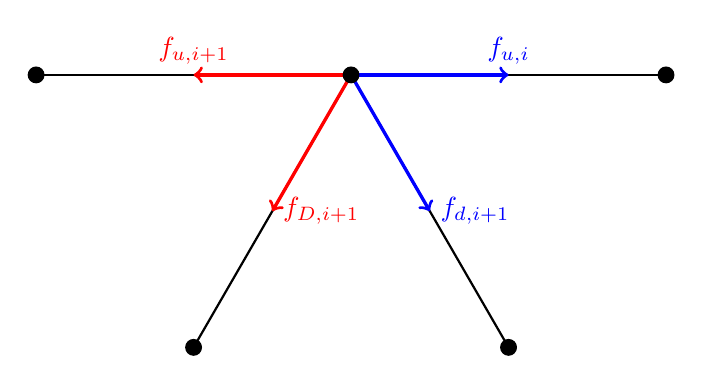
\begin{tikzpicture}[scale=2]
        \coordinate (A) at (0,0);
        \coordinate (B) at (1,1.73);
        \coordinate (C) at (2,0);
        \coordinate (D) at (3,1.73);
        \coordinate (E) at (4,0);
        \coordinate (F) at (5,1.73);


    
        \draw[thick] (D) -- (B);
        \draw[thick] (D) -- (C);
        \draw[thick] (D) -- (E);
        \draw[thick] (D) -- (F);

        \draw[very thick, blue, ->] (D) -- ($(D) !0.5! (F)$) node[above] {$f_{u,i}$};
        \draw[very thick, blue, ->] (D) -- ($(D) !0.5! (E)$) node[right] {$f_{d,i+1}$};
        \draw[very thick, red, ->] (D) -- ($(D) !0.5! (C)$) node[right] {$f_{D,i+1}$};
        \draw[very thick, red, ->] (D) -- ($(D) !0.5! (B)$) node[above] {$f_{u,i+1}$};


        \draw[fill=black] (B) circle (0.05) ;
        \draw[fill=black] (C) circle (0.05) ;
        \draw[fill=black] (D) circle (0.05) ;
        \draw[fill=black] (E) circle (0.05) ;
        \draw[fill=black] (F) circle (0.05) ;
    \end{tikzpicture}
\end{center}
Balancing the vertical forces, it's clear that since we only have two (symmetric) forces that have a component in the vertical direction, then we must demand that:
\begin{equation}
    f_{D,i+1} = -f_{d,i+1}
    \label{eq:f_d,i+2 = -f_d,i+1}
\end{equation}
and balancing horizontal forces, we have:
\begin{equation}
    \sum F_x = 0 \implies f_{u,i+1}=2f_{d,i+1}\cos(60^\circ)+f_{u,i}=f_{d,i+1}+f_{u,i}=\frac{2W_i}{\sqrt{3}}-f_{D,i}+f_{u,i}.
    \label{eq:}
\end{equation}
where I have made the substitution from equation \ref{eq:f_d,i+2 = -f_d,i+1}. We now have all the formulas we need to carry out teh recursion. Let us denote $i=0$ as the rightmost joint $M$, $K$ will be $i=1$, and so forth.

Our recursive equations are:
\begin{align}
    f_{d,i+1} &= \frac{2W_i}{\sqrt{3}}-f_{D,i} \\ 
    f_{D,i+1} &= -f_{d,i+1} \\
    f_{h,i+1} &= f_{h,i}+f_{D,i} - \frac{W_i}{\sqrt{3}} \\ 
    f_{u,i+1} &= \frac{2W_i}{\sqrt{3}}-f_{D,i}+f_{u,i}.
\end{align}Our boundary conditions are:
\begin{align}
    f_{d,0} &= 0 \\
    f_{D,0} &= 0 \\ 
    f_{h,0} &= 0 \\ 
    f_{u,0} &= 0
\end{align} 
and note that we take into account that the reaction force can be written as:
\begin{equation}
    W_0 = -875 \si{\kilo\newton}.
    \label{eq:}
\end{equation}
We can summarize the results in a table. Note that the forces to all the members denoted in proper notation in kilonewtons ir provided by the last four columns. The four previous columns serve no real purpose but for illustrative purposes (e.g. the forces calculated from the previous iteration now become the known force.):
\begin{center}
    \adjustbox{max width = \textwidth}{\begin{tabular}{|c|c|c|c|c|c||c|c|c|c|}
        \hline
        $i$ &
          $W_i$ &
          $f_{d,i}$ &
          $f_{D,i}$ &
          $f_{h,i}$ &
          $f_{u,i}$ &
          $f_{d,i+1}$ &
          $f_{D,i+1}$ &
          $f_{h,i+1}$ & 
          $f_{u,i+1}$ \\ 
        %
        \hline
        0 &
        -875 &
        0 &
        0 &
        0 &
        0 &
        $LM=-1010$ &
        $KL=1010$ &
        $KM=505$ &
        $JL=-1010$\\
        %

        1 &
        350 &
        $LM=-1010$ &
        $KL=1010$ &
        $KM=505$ &
        $JL=-1010$ &
        $JK=-606$ &
        $IJ=606$ &
        $IK=1313$ &
        $HJ=-1617$ \\

        2 &
        350 &
        $JK=-606$ &
        $IJ=606$ &
        $IK=1313$ &
        $HJ=-1617$ &
        $HI = -202$ &
        $GH = 202$ &
        $GI = 1718$ &
        $FH = -1819$ \\

        3 &
        350 &
        $HI = -202$ &
        $GH = 202$ &
        $GI = 1718$ &
        $FH = -1819$ &
        $FG = 202$ &
        $FE = -202$ &
        $EG = 1718$ &
        $DF = -1617$ \\

        4 &
        350 &
        $FG = 202$ &
        $FE = -202$ &
        $EG = 1718$ &
        $DF = -1617$ &
        $DE = 606$ &
        $CD = -606$ &
        $BE = 1313$ &
        $BD = -1010$ \\

        5 &
        350 &
        $DE = 606$ &
        $CD = -606$ &
        $BE = 1313$ &
        $BD = -1010$  &
        $BC = 1010$ &
        $AB = -1010$ &
        $AC = 500$ &
        $?B = 0$ \\
        \hline 
    \end{tabular}}
    \end{center}
    where $?B$ represents a hypothetical upper member had the pattern continued. It evaluates to zero, as it should, since nothing is there. Note that the system also has left-right symmetry. This should not come at a surprise since there is no horizontal force at $F$, so a person standing on the other side of the bridge should have the same force vectors as me if we follow the same method, even though our ``rightmost member'' does not agree!
    \vspace{2mm}
    
    This symmetry suggests that the horizontal reaction force from $A$ is zero. Indeed, if we look at the entire bridge as a system, it must maintain in equilibrium and the only possible horizontal external force is from $A$, which has to be zero. To verify, we note that the sum of $\vec{AB}+\vec{AC}=0$, or:
    \begin{equation}
        BC\cos(60^\circ) = AC
        \label{eq:}
    \end{equation}
    which is true if I take infinite significant digits, instead of rounding. The largest member in compression is $FH=-1819\times 10^3 \si{\newton}$, corresponding to a minimum moment of inertia of:
    \begin{equation}
        I = 3\frac{1819\times 10^3 \si{\newton} \cdot (5000 \si{\milli\meter})^2}{\pi^2 (200,000\si{\mega\pascal})} = 69.1 \times 10^6 \si{\milli\meter\tothe{4}}
        \label{eq:}
    \end{equation}
    And the minimum area is (when looking at stress):
    \begin{equation}
        A = 2\frac{1819\times 10^3\si{\newton}}{350\si{\mega\pascal}} = 10390\si{\milli\meter\squared}
    \end{equation}
    Looking at all HSS who have a second moment of inertia and an area of at least these values, the one with the lowest mass is $\boxed{\text{HSS 203x203x11}}$. As a quick check, we can calculate the radius of gyration to be:
    \begin{equation}
        r = \sqrt{\frac{I}{A}}=49.6\si{\milli\meter}
        \label{eq:}
    \end{equation}
    for this HSS, which is at least the value of $L/200=25.0\si{\milli\meter}$.

\newpage
\section{Problem Three: A not so bashy problem.}
\textbf{(a)} First, we can balance forces on the entire bridge. The total downwards force applied by the load is $F_\text{down}=11P$ and the upwards reaction $R$ from each end is the same, due to symmetry\footnote{Otherwise, balancing moments about the center of the bridge would yield a net moment}. Thus:
\begin{equation}
    2R=11P \implies R = \frac{11}{2}P
    \label{eq:R=11/2P}
\end{equation}
We can draw a free body diagram of the left roller:
\begin{center}
    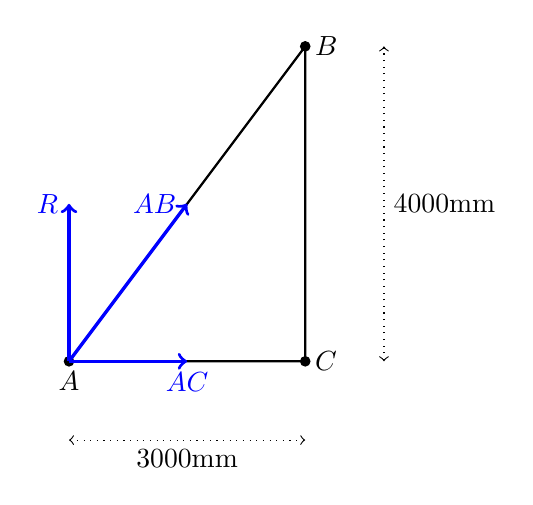
\begin{tikzpicture}
        \coordinate (A) at (0,0);
        \coordinate (C) at (3,0);
        \coordinate (B) at (3,4);

        \draw[fill=black] (A) circle (0.06) node[below] {$A$};
        \draw[fill=black] (C) circle (0.06) node[right] {$C$};
        \draw[fill=black] (B) circle (0.06) node[right] {$B$};

        \draw[thick] (A) -- (C) -- (B) -- (A);
        \draw[dotted, <->] (0,-1) -- (3,-1) node[midway,below] {$3000\si{\milli\meter}$};
        \draw[dotted, <->] (4,0) -- (4,4) node[midway,right] {$4000\si{\milli\meter}$};

        \draw[very thick, blue, ->] (A) -- ($(A) !0.5! (C)$) node[below]{$AC$};
        \draw[very thick, blue, ->] (A) -- ($(A) !0.5! (B)$) node[left] {$AB$};
        \draw[very thick, blue, ->] (A) -- ++(0, 2) node[left] {$R$};
    \end{tikzpicture}
\end{center}
Balancing forces in the vertical and horizontal directions gives us:
\begin{align}
    \sum F_y &= 0 \implies AB\frac{4}{\sqrt{3^2+4^2}} + R = 0 \implies AB = -\frac{5}{4}R \\
    \sum F_x &= 0 \implies AB\frac{3}{\sqrt{3^4+4^2}} + AB = 0 \implies AC =  - \frac{3}{4}AB.
    \label{eq:}
\end{align}
Substituting in the value of $R$ from equation \ref{eq:R=11/2P}, we get:
\begin{align}
    AB &= -\frac{55}{8}P \implies \boxed{F_{I} = -6.88P} \\
    AC &= \frac{165}{32}P
\end{align}
We can draw a free body diagram by cutting through members II and III to get:
\begin{center}
    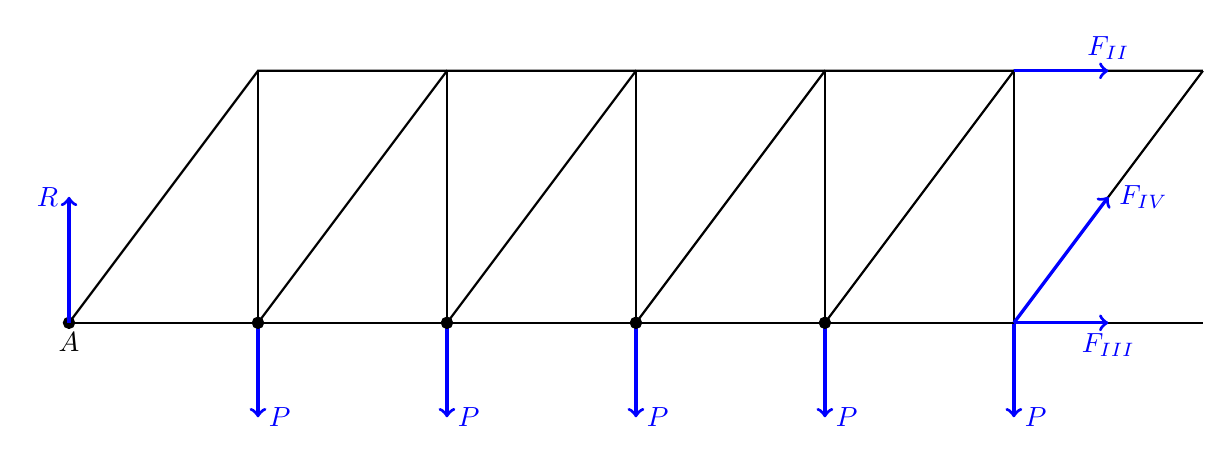
\begin{tikzpicture}[scale=0.8]
        \coordinate (A) at (0,0);
        \coordinate (C) at (3,0);
        \coordinate (B) at (3,4);
        \foreach \x in {0,3,6,...,12}{
            \draw[fill=black] (\x,0) circle (0.09);
            \draw[very thick,->,blue] (\x+3, 0) --++ (0,-1.5) node[right] {$P$};
            \draw[thick] (\x,0) -- (\x+3,0) -- (\x+3,4);
            \draw[thick] (\x,0) -- (\x+3,4) -- (\x+6,4);
        }
        \draw[thick] (15,0) -- (18,4);
        \draw[thick] (15,0) -- (18,0);
        \draw (0,0) node[below] {$A$}; 
        \draw[very thick, ->, blue] (15,0) -- (16.5,0) node[below] {$F_{III}$};
        \draw[very thick, ->, blue] (15,0) -- (16.5,2) node[right] {$F_{IV}$};
        \draw[very thick, ->, blue] (15,4) -- (16.5,4) node[above] {$F_{II}$};


        \draw[very thick, blue, ->] (A) -- ++(0, 2) node[left] {$R$};
    \end{tikzpicture}
\end{center}
Balancing vertical forces gives us:
\begin{align}
    \sum F_y &= 0 \implies 5P=F_{IV}\frac{4}{5}+R \label{eq:q3-fiv} \\
    \sum F_x &= 0 \implies F_{III} = -F_{II} - \frac{3}{5}F_{IV}
    \label{eq:q3-second-eq}
\end{align}
and a moment balance about $A$ gives:
\begin{equation}
    \sum M = 0 \implies P(3+6+9+12+15)+F_{II}(4)=\frac{4}{5}F_{IV}(15)
    \label{eq:q3-sum-of-moment}
\end{equation}
From equation \ref{eq:q3-fiv}, we can determine:
\begin{equation}
    F_{IV} = \frac{5}{4}\left(5P-\frac{11}{2}P\right) = - \frac{5}{8}P
    \label{eq:}
\end{equation}
which we can substitute in equation \ref{eq:q3-sum-of-moment} to get:
\begin{equation}
    F_{II}=\frac{1}{4}\left(-12\cdot \frac{5}{8}P - 45P\right) \implies \boxed{F_{II}=-13.13P}
    \label{eq:}
\end{equation}
and thus from equation \ref{eq:q3-second-eq}:
\begin{equation}
    F_{III} = 13.13P+\frac{3}{5}\frac{5}{8}P\implies \boxed{F_{III}=13.5P}.
    \label{eq:}
\end{equation}
is in tension. From the course notes, in order to prevent buckling, we must demand the force to be:
\begin{equation}
    F \le \frac{I\pi^2 E}{L^2} = \frac{(5.6\times 10^6\si{\milli\meter\tothe{4}})\pi^2(200,000\si{\mega\pascal})}{(3000\si{\milli\meter})^2} = 1228 \si{\kilo\newton}.
    \label{eq:}
\end{equation}
which corresponds to a $P$ value of:
\begin{equation}
    P = \frac{409\si{\kilo\newton}}{13.13}=93.6\si{\kilo\newton}.
    \label{eq:}
\end{equation}
Similarly, the member can also break from tensile or compressive forces, so the minimum force is:
\begin{equation}
    F \le \sigma_\text{yield}A = \frac{1}{2}(350\si{\mega\pascal})(2000\si{\milli\meter\squared}) = 700\si{\kilo\newton}
    \label{eq:}
\end{equation}
And since member $III$ always experiences the highest force, we have:
\begin{equation}
    P = \frac{700 \si{\kilo\newton}}{13.5} = 51.9\si{\kilo\newton}
    \label{eq:}
\end{equation}
Thus, members $II$ and $III$ will break at the same time at $\boxed{P=51.9\si{\kilo\newton}}$, assuming $\sigma_\text{yield}$ is the same for both compression and tension.

\newpage
\section{Problem Four: A Bracing Building}
We draw a free body diagram (not exciting at all):
\begin{center}
    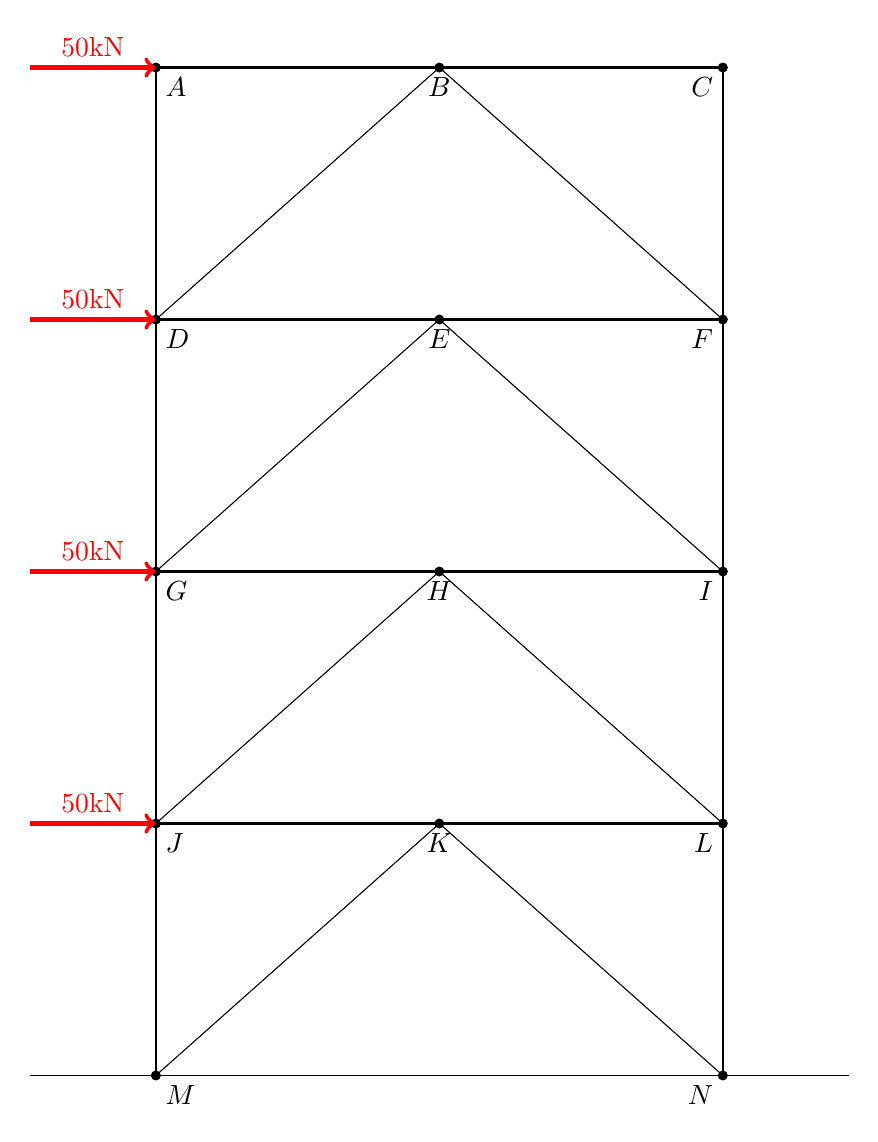
\begin{tikzpicture}[scale=0.8]
        \coordinate (M) at (0,0);
        \coordinate (N) at (9,0);
        \coordinate (J) at (0,4);
        \coordinate (K) at (4.5,4);
        \coordinate (L) at (9,4);
        \coordinate (G) at (0,8);
        \coordinate (H) at (4.5,8);
        \coordinate (I) at (9,8);
        \coordinate (D) at (0,12);
        \coordinate (E) at (4.5,12);
        \coordinate (F) at (9,12);
        \coordinate (A) at (0,16);
        \coordinate (B) at (4.5,16);
        \coordinate (C) at (9,16);

        \draw[fill=black] (A) circle (0.07) node[below right] {$A$};
        \draw[fill=black] (D) circle (0.07) node[below right] {$D$};
        \draw[fill=black] (G) circle (0.07) node[below right] {$G$};
        \draw[fill=black] (J) circle (0.07) node[below right] {$J$};
        \draw[fill=black] (M) circle (0.07) node[below right] {$M$};
        \draw[fill=black] (C) circle (0.07) node[below left] {$C$};
        \draw[fill=black] (F) circle (0.07) node[below left] {$F$};
        \draw[fill=black] (I) circle (0.07) node[below left] {$I$};
        \draw[fill=black] (L) circle (0.07) node[below left] {$L$};
        \draw[fill=black] (N) circle (0.07) node[below left] {$N$};
        \draw[fill=black] (B) circle (0.07) node[below] {$B$};
        \draw[fill=black] (E) circle (0.07) node[below] {$E$};
        \draw[fill=black] (H) circle (0.07) node[below] {$H$};
        \draw[fill=black] (K) circle (0.07) node[below] {$K$};

        \draw[thick] (M) -- (A) -- (C) -- (N);
        \draw[thick] (D) -- (F);
        \draw[thick] (G) -- (I);
        \draw[thick] (J) -- (L);

        \draw[] (M) -- (K) -- (N);
        \draw[] (J) -- (H) -- (L);
        \draw[] (G) -- (E) -- (I);
        \draw[] (D) -- (B) -- (F);

        \draw[] (-2,0) -- (11,0);

        \draw[red,ultra thick,<-] (A) -- ++(-2,0) node[midway,above] {$50\si{\kilo\newton}$};
        \draw[red,ultra thick,<-] (D) -- ++(-2,0) node[midway,above] {$50\si{\kilo\newton}$};
        \draw[red,ultra thick,<-] (G) -- ++(-2,0) node[midway,above] {$50\si{\kilo\newton}$};
        \draw[red,ultra thick,<-] (J) -- ++(-2,0) node[midway,above] {$50\si{\kilo\newton}$};
    \end{tikzpicture}
\end{center}
Wow, that's a lot to unpack! Let's begin by drawing a free body diagram for the top layer only:
\begin{center}
    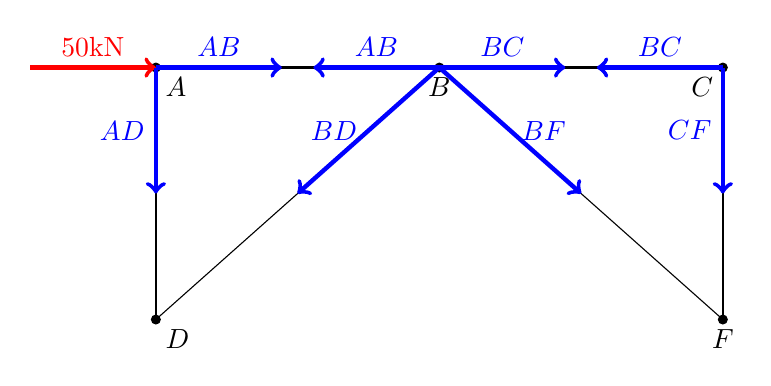
\begin{tikzpicture}[scale=0.8]
        \coordinate (D) at (0,12);
        \coordinate (F) at (9,12);
        \coordinate (A) at (0,16);
        \coordinate (B) at (4.5,16);
        \coordinate (C) at (9,16);

        \draw[fill=black] (A) circle (0.07) node[below right] {$A$};
        \draw[fill=black] (D) circle (0.07) node[below right] {$D$};
        \draw[fill=black] (C) circle (0.07) node[below left] {$C$};
        \draw[fill=black] (B) circle (0.07) node[below] {$B$};
        \draw[fill=black] (F) circle (0.07) node[below] {$F$};

        \draw[thick] (D) -- (A) -- (C) -- (F);
        \draw[] (D) -- (B) -- (F);

        \draw[red,ultra thick,<-] (A) -- ++(-2,0) node[midway,above] {$50\si{\kilo\newton}$};
        \draw[blue,ultra thick,->] (A) -- ++(2,0) node[midway,above] {$AB$};
        \draw[blue,ultra thick,->] (A) -- ++(0,-2) node[midway,left] {$AD$};
        \draw[blue,ultra thick,->] (B) -- ++(2,0) node[midway,above] {$BC$};
        \draw[blue,ultra thick,->] (B) -- ++(-2,0) node[midway,above] {$AB$};
        \draw[blue,ultra thick,->] (B) -- ($(B) !0.5! (F)$) node[midway,right] {$BF$};
        \draw[blue,ultra thick,->] (B) -- ($(B) !0.5! (D)$) node[midway,left] {$BD$};
        \draw[blue,ultra thick,->] (C) -- ++(-2,0) node[midway,above] {$BC$};
        \draw[blue,ultra thick,->] (C) -- ++(0,-2) node[midway,left] {$CF$};
    \end{tikzpicture}
\end{center}
Balancing vertical and horizontal forces at joint $A$, we have:
\begin{align}
    \sum F_y = 0 &\implies AD = 0 \\
    \sum F_x = 0 &\implies AB = -50\si{\kilo\newton}
\end{align}
Balancing vertical and horizontal forces at joint $C$, we have:
\begin{align}
    \sum F_y = 0 &\implies CF=0 \\ 
    \sum F_x = 0 &\implies BC=0
    \label{eq:}
\end{align}
Balancing forces at $B$ then gives:
\begin{align}
    \sum F_y = 0 &\implies BD\frac{4}{\sqrt{4^2+4.5^2}}=-BF\frac{4}{\sqrt{4^2+4.5^2}} \implies BD = -BF \\ 
    \sum F_x = 0 &\implies AB+BD\frac{4.5}{\sqrt{4^2+4.5^2}}=BC+BF\frac{4.5}{\sqrt{4^2+4.5^2}}
\end{align}
Using the previous results, we can write the sum of forces in the horizontal direction as:
\begin{equation}
    2BD\frac{4.5}{\sqrt{4.5^2+4^2}} = -AB \implies BD = 33.4\si{\kilo\newton}
    % 33.4488738
    \label{eq:}
\end{equation}
such that $BF=-33.4\si{\kilo\newton}$. Note that $AD$, $BC$, and $CF$ are zero force members. Therefore, I will neglect to draw their contributions in the next layer. A quicker method may actually be to draw them, and then recursively solve them, as I did for the other question. However for the sake of exercise, I'll write down all the steps (and draw them of course).
\begin{center}
    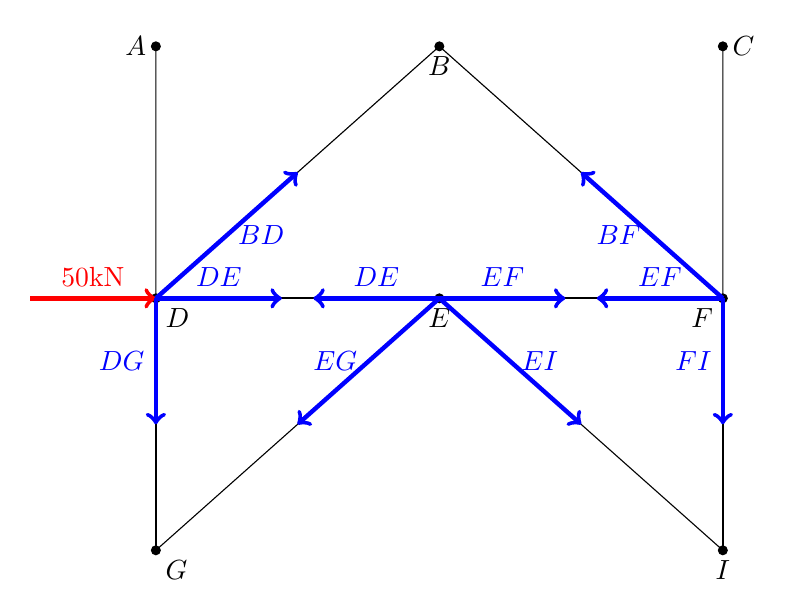
\begin{tikzpicture}[scale=0.8]
        \coordinate (D) at (0,12);
        \coordinate (F) at (9,12);
        \coordinate (A) at (0,16);
        \coordinate (B) at (4.5,16);
        \coordinate (C) at (9,16);
        \coordinate (X) at (0,20);
        \coordinate (Y) at (4.5,20);
        \coordinate (Z) at (9,20);

        \draw[fill=black] (A) circle (0.07) node[below right] {$D$};
        \draw[fill=black] (B) circle (0.07) node[below] {$E$};
        \draw[fill=black] (C) circle (0.07) node[below left] {$F$};
        \draw[fill=black] (D) circle (0.07) node[below right] {$G$};
        \draw[fill=black] (F) circle (0.07) node[below] {$I$};

        \draw[fill=black] (X) circle (0.07) node[left] {$A$};
        \draw[fill=black] (Y) circle (0.07) node[below] {$B$};
        \draw[fill=black] (Z) circle (0.07) node[right] {$C$};

        \draw[thick] (D) -- (A) -- (C) -- (F);
        \draw[] (X) -- (A) -- (Y) -- (C) -- (Z);
        \draw[] (D) -- (B) -- (F);

        \draw[red,ultra thick,<-] (A) -- ++(-2,0) node[midway,above] {$50\si{\kilo\newton}$};
        \draw[blue,ultra thick,->] (A) -- ++(2,0) node[midway,above] {$DE$};
        \draw[blue,ultra thick,->] (B) -- ++(-2,0) node[midway,above] {$DE$};
        \draw[blue,ultra thick,->] (C) -- ++(-2,0) node[midway,above] {$EF$};
        \draw[blue,ultra thick,->] (B) -- ++(2,0) node[midway,above] {$EF$};
        \draw[blue,ultra thick,->] (A) -- ++(0,-2) node[midway,left] {$DG$};
        \draw[blue,ultra thick,->] (B) -- ($(B) !0.5! (F)$) node[midway,right] {$EI$};
        \draw[blue,ultra thick,->] (B) -- ($(B) !0.5! (D)$) node[midway,left] {$EG$};
        \draw[blue,ultra thick,->] (A) -- ($(A) !0.5! (Y)$) node[midway,right] {$BD$};
        \draw[blue,ultra thick,->] (C) -- ($(C) !0.5! (Y)$) node[midway,left] {$BF$};
        \draw[blue,ultra thick,->] (C) -- ++(0,-2) node[midway,left] {$FI$};
    \end{tikzpicture}
\end{center}
We do the same thing, balancing forces on $D$, then $F$, then $E$ to get:
\begin{align}
    \sum F_y = 0 &\implies DG=BD\frac{4}{\sqrt{4.5^2+4^2}} = 22.2\si{\kilo\newton} \\%-22.222222222 \\ 
    \sum F_x = 0 &\implies 50+DE+BD\frac{4.5}{\sqrt{4.5^2+4^2}} = 0 \implies DE = -(BD\frac{4.5}{\sqrt{4.5^2+4^2}}+50) = -75\si{\kilo\newton} % 27.777777777
\end{align}
For joint $F$:
\begin{align}
    \sum F_y = 0 &\implies FI=BF\frac{4}{\sqrt{4.5^2+4^2}} = -22.2\si{\kilo\newton} \\%22.22222222
    \sum F_x = 0 &\implies EF = -BF\frac{4.5}{\sqrt{4.5^2+4^2}} = 25.0\si{\kilo\newton}
\end{align}
For joint $E$:
\begin{align}
    \sum F_y = 0 &\implies EG=-EI \\ 
    \sum F_x = 0 &\implies DE+EG\frac{4.5}{\sqrt{4.5^2+4^2}}=EF+DI\frac{4.5}{\sqrt{4.5^2+4^2}}
\end{align}
where the last equation can again be written as:
\begin{equation}
    2EG\frac{4.5}{\sqrt{4.5^2+4^2}} = EF-DE \implies EG = 66.9\si{\kilo\newton} 
    % 35.3071446
    \label{eq:}
\end{equation}
and again, we have $EI=-EG$. We can then draw a free body diagram of the third layer:
\begin{center}
    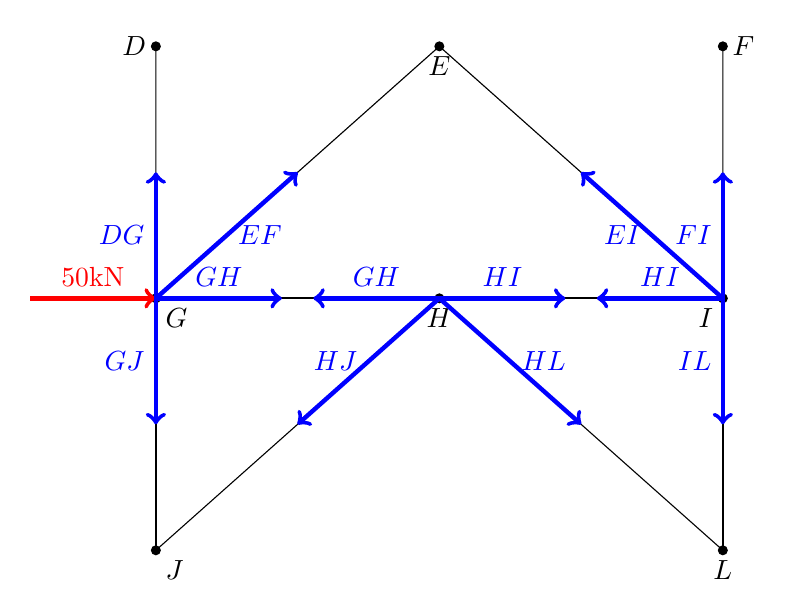
\begin{tikzpicture}[scale=0.8]
        \coordinate (D) at (0,12);
        \coordinate (F) at (9,12);
        \coordinate (A) at (0,16);
        \coordinate (B) at (4.5,16);
        \coordinate (C) at (9,16);
        \coordinate (X) at (0,20);
        \coordinate (Y) at (4.5,20);
        \coordinate (Z) at (9,20);

        \draw[fill=black] (A) circle (0.07) node[below right] {$G$};
        \draw[fill=black] (B) circle (0.07) node[below] {$H$};
        \draw[fill=black] (C) circle (0.07) node[below left] {$I$};
        \draw[fill=black] (D) circle (0.07) node[below right] {$J$};
        \draw[fill=black] (F) circle (0.07) node[below] {$L$};

        \draw[fill=black] (X) circle (0.07) node[left] {$D$};
        \draw[fill=black] (Y) circle (0.07) node[below] {$E$};
        \draw[fill=black] (Z) circle (0.07) node[right] {$F$};

        \draw[thick] (D) -- (A) -- (C) -- (F);
        \draw[] (X) -- (A) -- (Y) -- (C) -- (Z);
        \draw[] (D) -- (B) -- (F);

        \draw[red,ultra thick,<-] (A) -- ++(-2,0) node[midway,above] {$50\si{\kilo\newton}$};
        \draw[blue,ultra thick,->] (A) -- ++(2,0) node[midway,above] {$GH$};
        \draw[blue,ultra thick,->] (B) -- ++(-2,0) node[midway,above] {$GH$};
        \draw[blue,ultra thick,->] (C) -- ++(-2,0) node[midway,above] {$HI$};
        \draw[blue,ultra thick,->] (B) -- ++(2,0) node[midway,above] {$HI$};
        \draw[blue,ultra thick,->] (A) -- ++(0,-2) node[midway,left] {$GJ$};
        \draw[blue,ultra thick,->] (A) -- ++(0,2) node[midway,left] {$DG$};
        \draw[blue,ultra thick,->] (C) -- ++(0,-2) node[midway,left] {$IL$};
        \draw[blue,ultra thick,->] (C) -- ++(0,2) node[midway,left] {$FI$};

        \draw[blue,ultra thick,->] (B) -- ($(B) !0.5! (F)$) node[midway,right] {$HL$};
        \draw[blue,ultra thick,->] (B) -- ($(B) !0.5! (D)$) node[midway,left] {$HJ$};
        \draw[blue,ultra thick,->] (A) -- ($(A) !0.5! (Y)$) node[midway,right] {$EF$};
        \draw[blue,ultra thick,->] (C) -- ($(C) !0.5! (Y)$) node[midway,left] {$EI$};
    \end{tikzpicture}
\end{center}
We do the same thing, balancing forces on $G$, then $I$, then $H$ to get:
\begin{align}
    \sum F_y = 0 &\implies GJ=DG+EG\frac{4}{\sqrt{4.5^2+4^2}} = 66.7\si{\kilo\newton} \\ 
    \sum F_x = 0 &\implies GH = -\left(50+EG\frac{4.5}{\sqrt{4.5^2+4^2}}\right) = -100\si{\kilo\newton}
\end{align}
And balancing forces on $I$ to get:
\begin{align}
    \sum F_y = 0 &\implies IL=FI+EI\frac{4}{\sqrt{4.5^2+4^2}} = -66.7\si{\kilo\newton} \\ 
    \sum F_x = 0 &\implies HI = -EI\frac{4.5}{\sqrt{4.5^2+4^2}} = 50\si{\kilo\newton}
\end{align}
For joint $H$:
\begin{align}
    \sum F_y = 0 &\implies HJ = - HL \\ 
    \sum F_x = 0 &\implies HJ = \left(HI-GH\right)\frac{\sqrt{4.5^2+4^2}}{9} = 100.3\si{\kilo\newton}
\end{align}
and similarly $HL=-100.3\si{\kilo\newton}$. We can draw the free body diagram for the first floor:
\begin{center}
    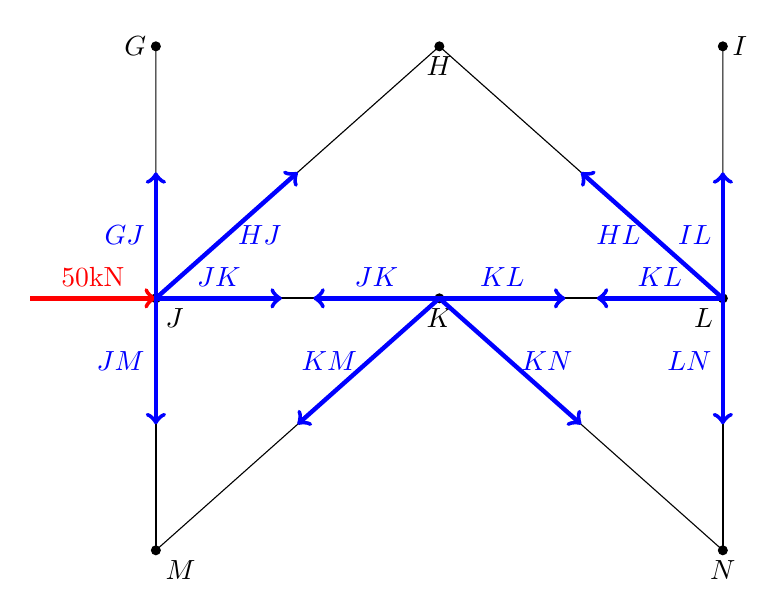
\begin{tikzpicture}[scale=0.8]
        \coordinate (D) at (0,12);
        \coordinate (F) at (9,12);
        \coordinate (A) at (0,16);
        \coordinate (B) at (4.5,16);
        \coordinate (C) at (9,16);
        \coordinate (X) at (0,20);
        \coordinate (Y) at (4.5,20);
        \coordinate (Z) at (9,20);

        \draw[fill=black] (A) circle (0.07) node[below right] {$J$};
        \draw[fill=black] (B) circle (0.07) node[below] {$K$};
        \draw[fill=black] (C) circle (0.07) node[below left] {$L$};
        \draw[fill=black] (D) circle (0.07) node[below right] {$M$};
        \draw[fill=black] (F) circle (0.07) node[below] {$N$};

        \draw[fill=black] (X) circle (0.07) node[left] {$G$};
        \draw[fill=black] (Y) circle (0.07) node[below] {$H$};
        \draw[fill=black] (Z) circle (0.07) node[right] {$I$};

        \draw[thick] (D) -- (A) -- (C) -- (F);
        \draw[] (X) -- (A) -- (Y) -- (C) -- (Z);
        \draw[] (D) -- (B) -- (F);

        \draw[red,ultra thick,<-] (A) -- ++(-2,0) node[midway,above] {$50\si{\kilo\newton}$};
        \draw[blue,ultra thick,->] (A) -- ++(2,0) node[midway,above] {$JK$};
        \draw[blue,ultra thick,->] (B) -- ++(-2,0) node[midway,above] {$JK$};
        \draw[blue,ultra thick,->] (C) -- ++(-2,0) node[midway,above] {$KL$};
        \draw[blue,ultra thick,->] (B) -- ++(2,0) node[midway,above] {$KL$};
        \draw[blue,ultra thick,->] (A) -- ++(0,-2) node[midway,left] {$JM$};
        \draw[blue,ultra thick,->] (A) -- ++(0,2) node[midway,left] {$GJ$};
        \draw[blue,ultra thick,->] (C) -- ++(0,-2) node[midway,left] {$LN$};
        \draw[blue,ultra thick,->] (C) -- ++(0,2) node[midway,left] {$IL$};

        \draw[blue,ultra thick,->] (B) -- ($(B) !0.5! (F)$) node[midway,right] {$KN$};
        \draw[blue,ultra thick,->] (B) -- ($(B) !0.5! (D)$) node[midway,left] {$KM$};
        \draw[blue,ultra thick,->] (A) -- ($(A) !0.5! (Y)$) node[midway,right] {$HJ$};
        \draw[blue,ultra thick,->] (C) -- ($(C) !0.5! (Y)$) node[midway,left] {$HL$};
    \end{tikzpicture}
\end{center}
We do the same thing, balancing forces on $J$, then $L$, then $K$ to get:
\begin{align}
    \sum F_y = 0 &\implies JM=GJ+HJ\frac{4}{\sqrt{4.5^2+4^2}} = 133.3\si{\kilo\newton} \\ 
    \sum F_x = 0 &\implies JK = -\left(50+HJ\frac{4.5}{\sqrt{4.5^2+4^2}}\right) = -125\si{\kilo\newton}
\end{align}
And balancing forces on $L$ to get:
\begin{align}
    \sum F_y = 0 &\implies LN=IL+HL\frac{4}{\sqrt{4.5^2+4^2}} = -133.3 \si{\kilo\newton} \\ 
    \sum F_x = 0 &\implies KL = -HL\frac{4.5}{\sqrt{4.5^2+4^2}} = 75\si{\kilo\newton}
\end{align}
For joint $K$:
\begin{align}
    \sum F_y = 0 &\implies KM = - KN \\ 
    \sum F_x = 0 &\implies KM = \left(KL-JK\right)\frac{\sqrt{4.5^2+4^2}}{9} = 133.8\si{\kilo\newton}
\end{align}
and similarly $F_{KN}=-133.8\si{\kilo\newton}$
We can summarize everything in a table, where all forces are in units of kilonewtons.
\begin{center}
    \begin{tabular}{|c|c|c|c|c|c|c|}
        \hline
        Story & Left Vertical & Right Vertical & Left Top  & Right Top & Left Diagonal & Right Diagonal \\ \hline
        4     & $AD=0$        & $CF=0$         & $AB=-50$  & $BC=0$    & $BD=33.4$     & $BF=-33.4$     \\ \hline
        3     & $DG=22.2$     & $FI=-22.2$     & $DE=-75$  & $EF=25$   & $EG=66.9$        & $EI=-66.9$     \\ \hline
        2     & $GJ=66.7$     & $IL=-66.7$     & $GH=-100$ & $HI=50$   & $HJ=100.3$    & $HL=-100.3$    \\ \hline
        1     & $JM=133.3$    & $LN=-133.3$    & $JK=-125$ & $KL=75$   & $KM=133.8$    & $KN=-133.8$    \\ \hline
    \end{tabular}
\end{center}
The largest member in compression is $KN=-133.8\times 10^3 \si{\newton}$ (which also happens to be the longest, so we don't need to look at other shorter lengths), corresponding to a minimum moment of inertia of:
    \begin{equation}
        I \ge 3\frac{133.8\times 10^3 \si{\newton} \cdot \left[(4000 \si{\milli\meter})^2+(4500 \si{\milli\meter})^2\right]}{\pi^2 (200,000\si{\mega\pascal})} = 7.37 \times 10^6 \si{\milli\meter\tothe{4}}
        \label{eq:}
    \end{equation}
    And the minimum area is (when looking at stress):
    \begin{equation}
        A \ge 2\frac{133.8\times 10^3\si{\newton}}{350\si{\mega\pascal}} = 765\si{\milli\meter\squared}
    \end{equation}
    Looking at all HSS who have a second moment of inertia and an area of at least these values, the one with the lowest mass is $\boxed{\text{HSS 152x152x4.8}}$. As a quick check, we can calculate the radius of gyration to be:
    \begin{equation}
        r = \sqrt{\frac{I}{A}}=59.9\si{\milli\meter}
        \label{eq:}
    \end{equation}
    for this HSS, which is at least the value of $L/200=30.1\si{\milli\meter}$.
    % Desmos Notebook: https://www.desmos.com/calculator/1lcnexxeb5
    \end{document}
